%
% geometrie.tex %% Beispiele partieller Differentialgleichungen 
%
% (c) 2008 Prof Dr Andreas Mueller
%
\begin{figure}
\centering
\begin{tabular}{cc}
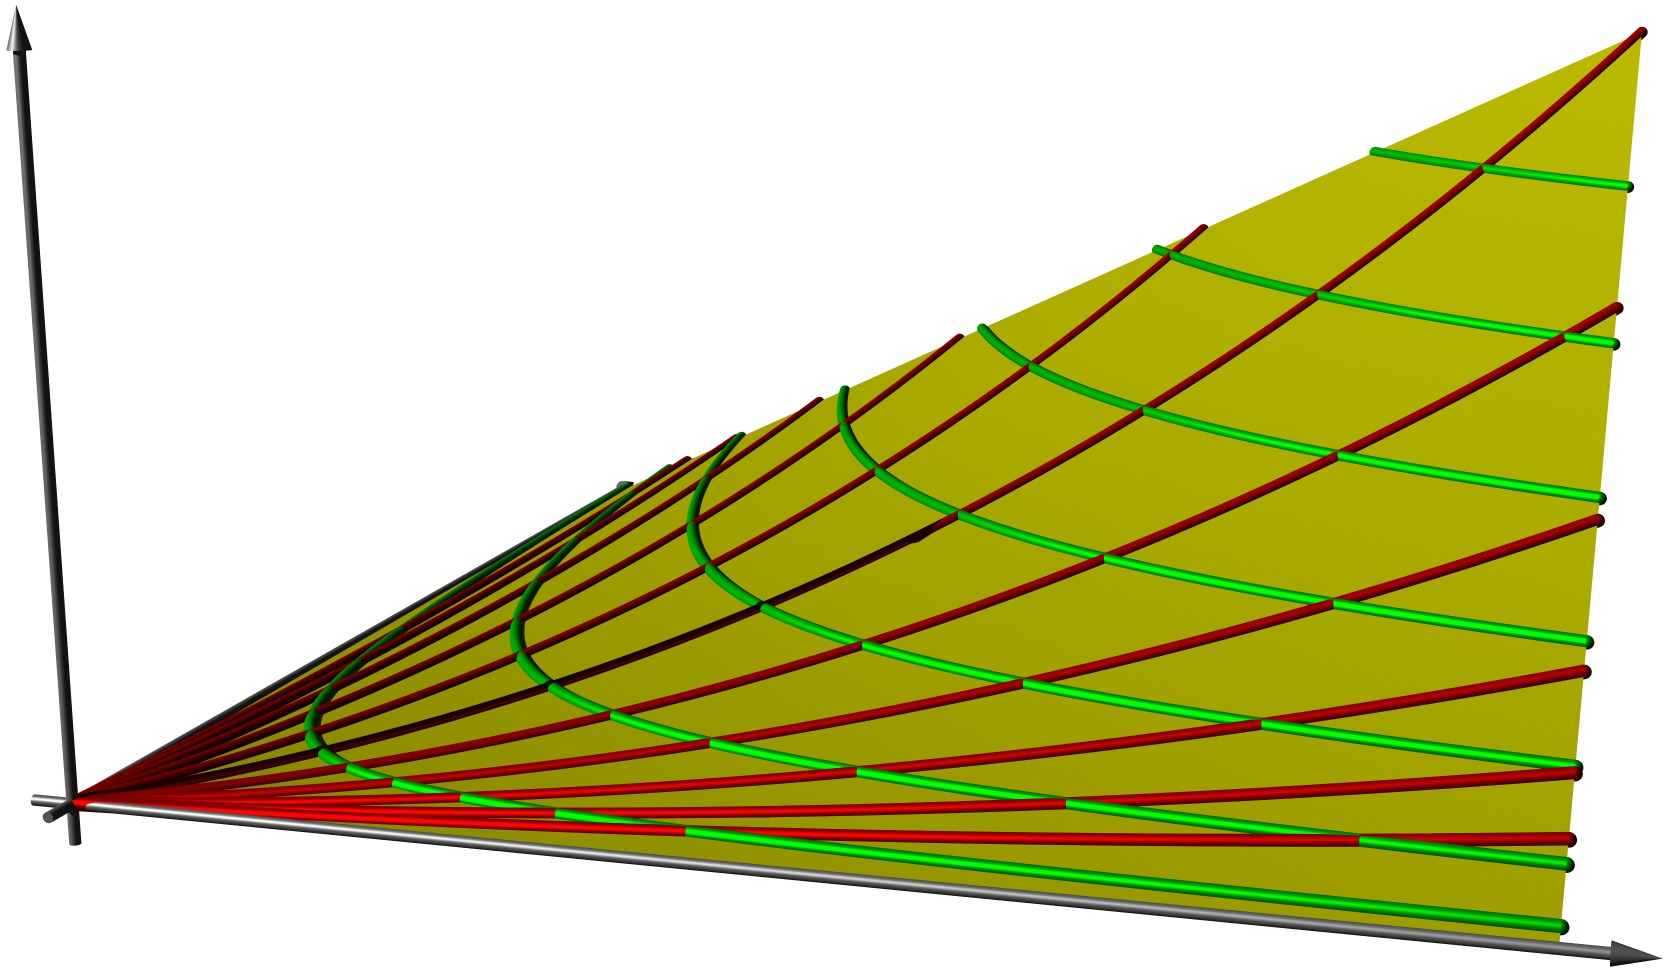
\includegraphics[width=0.6\hsize]{../common/3d/surface.jpg}&%
\includegraphics[width=0.35\hsize]{../common/images/kurven-1.pdf}
\end{tabular}
\caption{The surface create as the graph of $z=f(x,y)$ with $f(x,y)=xy$
can also be seen as the union of the red and green stets of curves
The surface has the parametrization \eqref{quasliniear:flaechebeispiel}.
The green curves are coordinate lines with $s=\operatorname{const}$,
the red curves are are coordinate lines with $t=\operatorname{const}$.
On the left the representation as a surface, on the right the coordinate
lines
${\color{red}t}=\operatorname{const}$
and
${\color{green}s}=\operatorname{const}$
projected to the $x$-$y$-plane.
\label{quasilinear:flaechenalskurven}
}
\end{figure}

\section{Curves on the solution surface}
\rhead{Curves on the solution surface}
The surface undoubtedly is a twodimensional which normally can only be dealt
with using partial derivatives.
Nevertheless, our best chance to solve a differential equation is to 
reduce it to an ordinary differential equation where we have plenty
of techniques to solve the equation.
So we try to find the solution surface ``curve by curve'', i.~e.~to describe
it as a bunch of curves.

\subsubsection{Solution surface as a set of curves}
The graph of the function $u(x,y)$ can be considered as a set of curves
in two obvious ways.
On the one hand, there is the set of curves $x\mapsto u(x,y)$ parametrized
by $y$, on the other hand there is a set of curves $y\mapsto u(x,y)$
parametrized by $x$.
These parametrizations aren't very useful, as the derivatives of these
curves are just the partial derivatives.
However, there are infinitely many parametrizations of the form
\begin{equation}
(s,t)\mapsto \vec x(s,t)
=
\begin{pmatrix}x(s,t)\\y(s,t)\\z(s,t)\end{pmatrix}
\label{quasilinear:kurvenschar}
\end{equation}
which we can consider as the set of curves $t\mapsto \vec x(s,t)$
parametrized by $s$ and as the set of curves $s\mapsto\vec x(s,t)$
parametrized by $t$.
Derivatives of these parametrizations give combinations of linear 
with a better chance for us to link them to the differential equation
at hand.

\begin{beispiel}
Figure~\ref{quasilinear:flaechenalskurven} shows the graph of the function
$u(x,y)=xy$.
An alternative parametrization is
\begin{equation}
(t,s)
\mapsto
\begin{pmatrix}x\\y\\z\end{pmatrix}
=
\begin{pmatrix}t\sqrt{s}\\\frac1t\sqrt{s}\\s\end{pmatrix}.
\label{quasliniear:flaechebeispiel}
\end{equation}
In fact, $xy = t\sqrt{s}\frac1t\sqrt{s}=s=z$.
The resulting sets of curves are displayed as red and green curves
in figure~\ref{quasilinear:flaechenalskurven}.
\end{beispiel}

On the other hand, given a set of curves, we can in many cases recover
a function $u(x,y)$ in such a way that the graph of $u$ is the same
surface.
For this we have to solve the equations
\begin{align*}
x(s(x,y),t(x,y))&=x\\
y(s(x,y),t(x,y))&=y
\end{align*}
for any point $(x,y)$ we have to solve the equations.
With the functions $s(x,y)$ and $t(x,y)$ determined, we can set
\[
u(x,y)=z(s(x,y), t(x,y)).
\]
Thus the goal in solving a partial differential equation is to find
a set of curves \eqref{quasilinear:kurvenschar} that forms the surface.

\begin{beispiel}
\begin{figure}
\centering
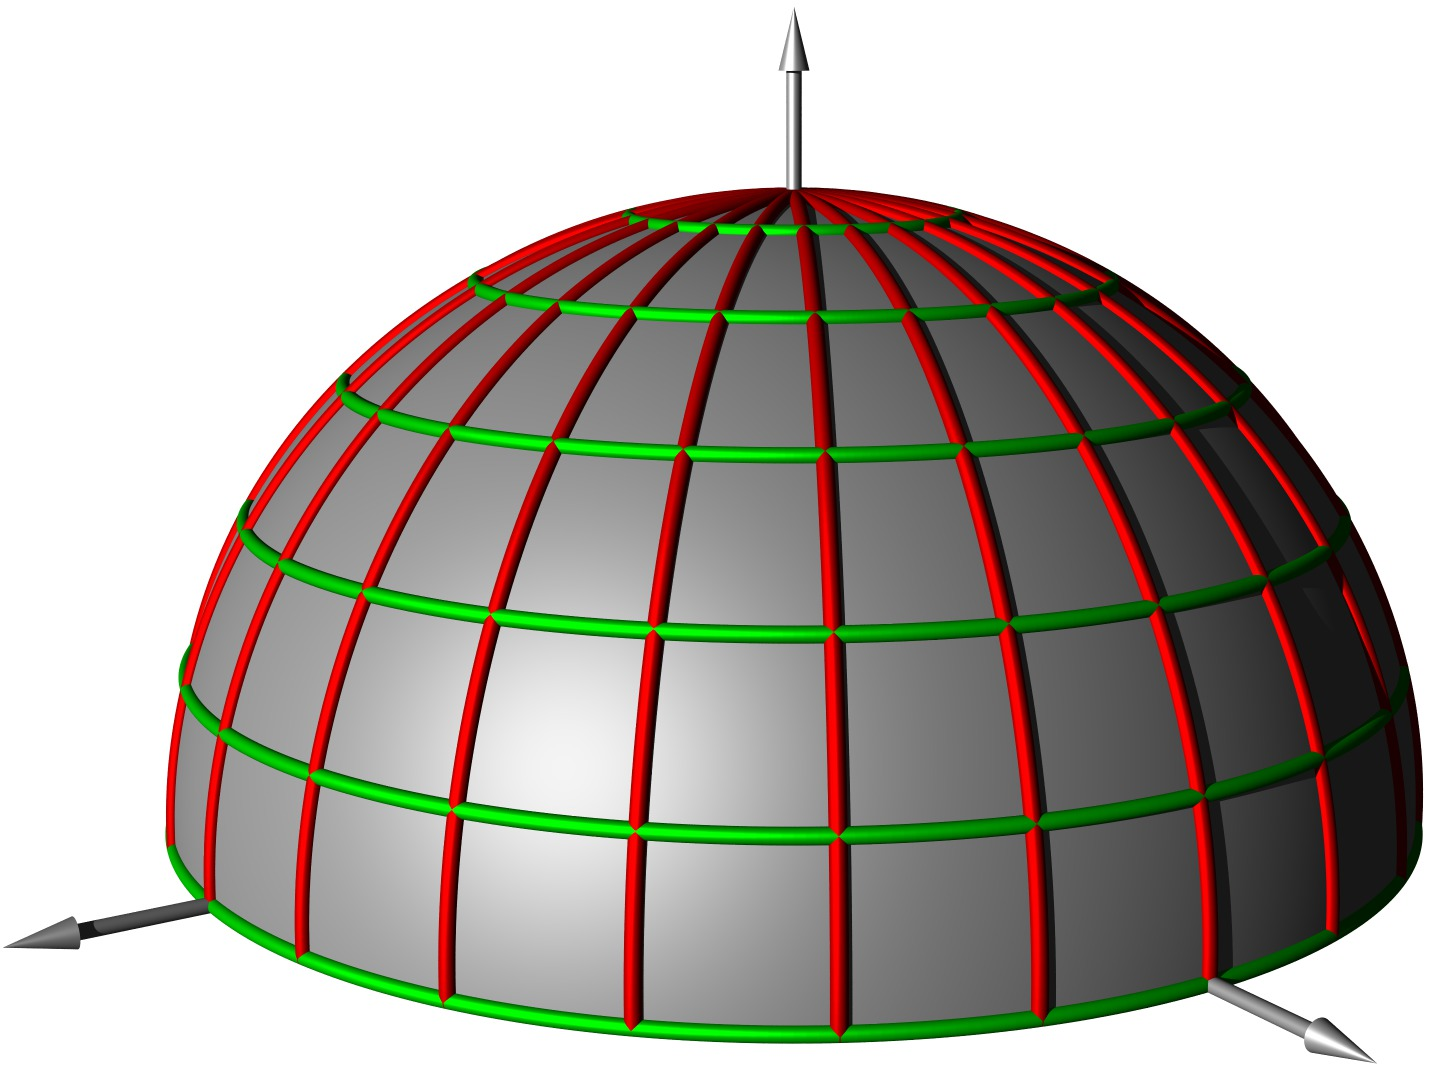
\includegraphics[width=0.8\hsize]{../common/3d/kugel.jpg}
\caption{Representation of a half sphere as two sets of curves
\label{quasilinear:kugel}}
\end{figure}
The parametrization
\[
(\vartheta,\varphi)\mapsto
\begin{pmatrix}
\sin\vartheta\cos\varphi\\
\sin\vartheta\sin\varphi\\
\cos\vartheta
\end{pmatrix}
\]
describes the half sphere (figure~\ref{quasilinear:kugel}).
for $0\le\varphi\le 2\pi$ and $0\le \vartheta\le \frac{\pi}2$
(Abbildung~\ref{quasilinear:kugel}).

The curves
\[
\vartheta\mapsto
\begin{pmatrix}
\sin\vartheta\cos\varphi\\
\sin\vartheta\sin\varphi\\
\cos\vartheta
\end{pmatrix}
\qquad
\text{und}
\qquad
\varphi\mapsto
\begin{pmatrix}
\sin\vartheta\cos\varphi\\
\sin\vartheta\sin\varphi\\
\cos\vartheta
\end{pmatrix}
\]
are on the left curves with curve parameter $\vartheta$, parametrized
by the longitude $\varphi$, and on the right, the curve parameter is
$\varphi$, and the set of curves is parametrized by the latitude $\vartheta$.

The equations
\begin{align*}
x&=\sin\vartheta\cos\varphi\\
y&=\sin\vartheta\sin\varphi\\
\end{align*}
can be solved, at least for $x\ne 0$, by
\begin{align*}
\tan\varphi&=\frac{y}{x}\\
\sin\vartheta &=\sqrt{x^2+y^2}.
\end{align*}
This is enough to construct the function $u(x,y)$:
\[
u=\cos\vartheta=\sqrt{1-\sin^2\vartheta}=\sqrt{1-x^2-y^2}.
\qedhere
\]
\end{beispiel}

So the goal is to construct a parametrization of the solution surface
with some more or less arbitrary parameters that allow to reduce the
partial differential equation into some parametrized ordinary
differential equation which can then be solved using traditional methods.
Our first task is to identify the parameters.

\subsubsection{First Parameter: Cauchy initial values}
\begin{figure}
\begin{center}
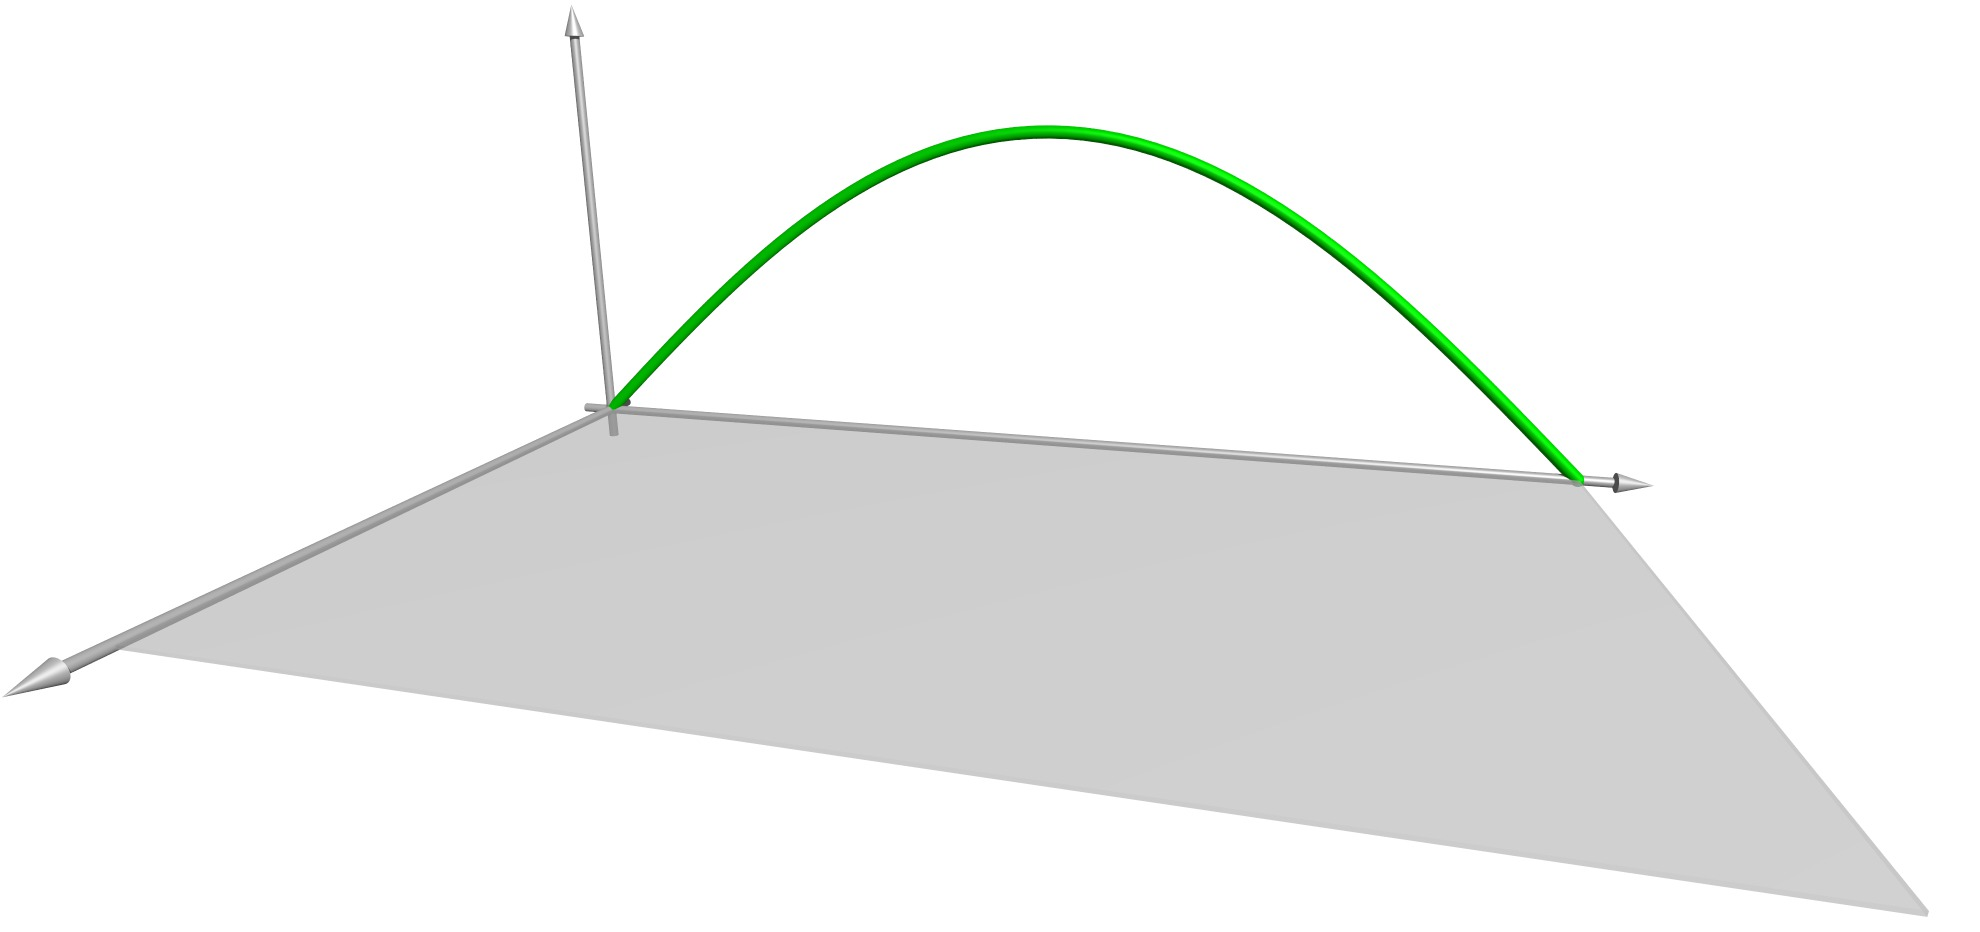
\includegraphics[width=\hsize]{../common/3d/cauchy.jpg}
\end{center}
\caption{Cauchy initial durve of a partial differential
($y$-Achse nach rechts)
\label{geometrie:cauchy-anfangskurve}}
\end{figure}
We want to solve the Cauchy initial problem for a partial differential
equation of first order.
This means that the initial curve of the solution is already given
(see figure~\ref{geometrie:cauchy-anfangskurve}).
It is specified as the curve
\begin{equation}
s\mapsto\vec x_0(s)=\begin{pmatrix}
x_0(s)\\
y_0(s)\\
z_0(s)
\end{pmatrix},
\label{quasilinear:anfangskurve}
\end{equation}
parametrized by $s$.
The solution function $u(x,y)$ we are looking must satisfy
the condition
\[
u(x_0(s), y_0(s))=z_0(s)
\]
for each $s$.

\subsubsection{Second parameter: curve parameter}
We have to extend this initial curve to a set of curves with a
second parameter to get something like \eqref{quasilinear:kurvenschar}.
Für $t=0$ muss die Anfangskurve entstehen:
\[
\vec x(s,0)=x_0(s).
\]
Each curve $t\mapsto \vec x(s,t)$ is a curve with initial point $x_0(s)$.
This suggest that we may find these curves as solutions of an ordinary
differential equation with parameter $t$, which then naturally becomes
the curve parameter.

\subsection{Quasilinear partial differential equations of first order}
In this section, wie only consider a quasilinear partial differential
equation of the form
\begin{equation}
a\frac{\partial u}{\partial x}
+
b\frac{\partial u}{\partial y}
=
c.
\label{quasilinear:equation}
\end{equation}
We want to show that for this type of differential equation, the
Cauchy problem can be solved most of the time and we want to undertand
the circumstances when it isn't.

\subsubsection{Ordinary differential equation of first order}
We quickly recall what the solution of an ordinary differential equation
of first order means.
Such an equation is supposed to fix a function $y(x)$ in such a way
that the derivative $y'(x)$ is given by the coordinates $(x,y)$
\[
y'=f(x,y).
\]
Geometrically, the function $f(x,y)$ specifies a direction field,
and the graph of the solution function is tangent to direction
field everywhere.

To find the solution curves, on progresses as follows.
The initial condition $y(0)=y_0$ fixes one point of the solution
curve.
The differential equation then determines the slope in that point
as $y'(0)=f(0,y(0))$.
A first approximation for a neighboring point $y(h)$ would then be
\begin{equation}
y(h)=y(0)+f(0,y(0))\cdot h.
\label{quasilinear:euler}
\end{equation}
Iterating this procedure we can obtain $y(2h)$, $y(3h)$,$\dots$.
Of course, these are not precise values, but it can be shown that
the represent the true solution rather well, and in many cases
converge to the true solution when $h\to 0$.
This explains why ordinary differential equations of this form have
unique solutions under very mild conditions and why a single
initial value sufficies to determine that solution.

\subsubsection{Existence of solutions}
We try to translate the argument for the existence of a solution to
an equation of the form \eqref{quasilinear:equation}.
We now have two partial derivatives that are linked by the equation
\eqref{quasilinear:equation}, which on its own does not determine
them both.
As a linear equation for the derivatives of $u$ at a given point
$(x,y,u(x,y))$
\eqref{quasilinear:equation} has infinitely many solutions.

But not all is lost.
Since we want to solve the Cauchy problem, we already know the 
values of the function along the initial curve.
We have in some sense infinitely many initial values.
To simplify the discussion, we assume that the we know initial values
$u(0,y) = g(y)$ along the $y$ axis and have to find a solution in the domain
$x>0$.
But this means that we also know the partial derivative
\[
\frac{\partial u}{\partial y}(0,y) = g'(y)
\]
of $u$ with respect to $y$.

Now if the coefficient $a(x,y,u)$ in \eqref{quasilinear:equation}
is different from $0$, we can solve the equation for $\partial_x u$.
This means that the partial differential equation deterines one of
the partial derivatives given the other.
The initial values and derivatives along the initial curve determine
the partial derivatives normal to the boundary, we know both derivatives.

This means we are in a situation quite similar to the ordinary
differential equation.
Using the partial derivative in the $x$ direction, we can find
$u(h,y)$ as
\[
u(h,y) = g(y) + h\frac{\partial u}{\partial x}(0,y)
\]
for small $h$.
This determines all the values of the function on the line $x=h$,
and thus the partial derivatives with respect to $x$.
Iterating this procedure, we can get an approximate solution
which will in many cases converge to the exact solution when $h\to 0$.

This argument allows to be confident that a quasilinear partial
differential equation will in fact have a solution that we can expect
to find from ordinary differential equations.
Our next step is thus to construct such an equation.

\subsubsection{Vector form of the differential equation}
The solution can be simplify using the following geometric consideration.
Again we view the solution function $u(x,y)$ as a graph in a three dimensional
coordinate system $(x,y,u)$.
The partial differential equation \eqref{quasilinear:equation}
can be written as a vector equation
\begin{equation}
\begin{pmatrix}a\\b\\c\end{pmatrix}
\cdot
\begin{pmatrix}
\frac{\partial u}{\partial x}\\
\frac{\partial u}{\partial y}\\
-1
\end{pmatrix}
=0,
\label{quasilinear:vektorform}
\end{equation}
as one can convince oneself by multiplying out.
We denote the vector on the left as
\[
\vec v=\begin{pmatrix}
a(x,y,u)\\
b(x,y,u)\\
c(x,y,u)
\end{pmatrix}.
\]
The vector on the right
\[
\vec n=
\begin{pmatrix}
\frac{\partial u}{\partial x}\\
\frac{\partial u}{\partial y}\\
-1
\end{pmatrix}
\]
Is normal to the graph of the function $z=u(x,y)$.
To see this, consider the tangent vectors of the surface in the
direction of the $x$ and $y$ coordinates.
They are
\[
\vec t_x
=
\begin{pmatrix}1\\0\\\frac{\partial u}{\partial x}\end{pmatrix}
\qquad
\text{and}
\qquad
\vec t_y
=
\begin{pmatrix}0\\1\\\frac{\partial u}{\partial y}\end{pmatrix}.
\]
The scalar product of $\vec n$ with the vectors $\vec{t}_x$ and $\vec{t}_y$
is:
\[
\vec n\cdot\vec t_x
=
\begin{pmatrix}
\frac{\partial u}{\partial x}\\
\frac{\partial u}{\partial y}\\
-1
\end{pmatrix}
\cdot
\begin{pmatrix}1\\0\\\frac{\partial u}{\partial x}\end{pmatrix}
=0
\qquad
\text{and}
\qquad
\vec n\cdot\vec t_y
=
\begin{pmatrix}
\frac{\partial u}{\partial x}\\
\frac{\partial u}{\partial y}\\
-1
\end{pmatrix}
\cdot
\begin{pmatrix}0\\1\\\frac{\partial u}{\partial y}\end{pmatrix}
=0.
\]
\begin{figure}
\begin{center}
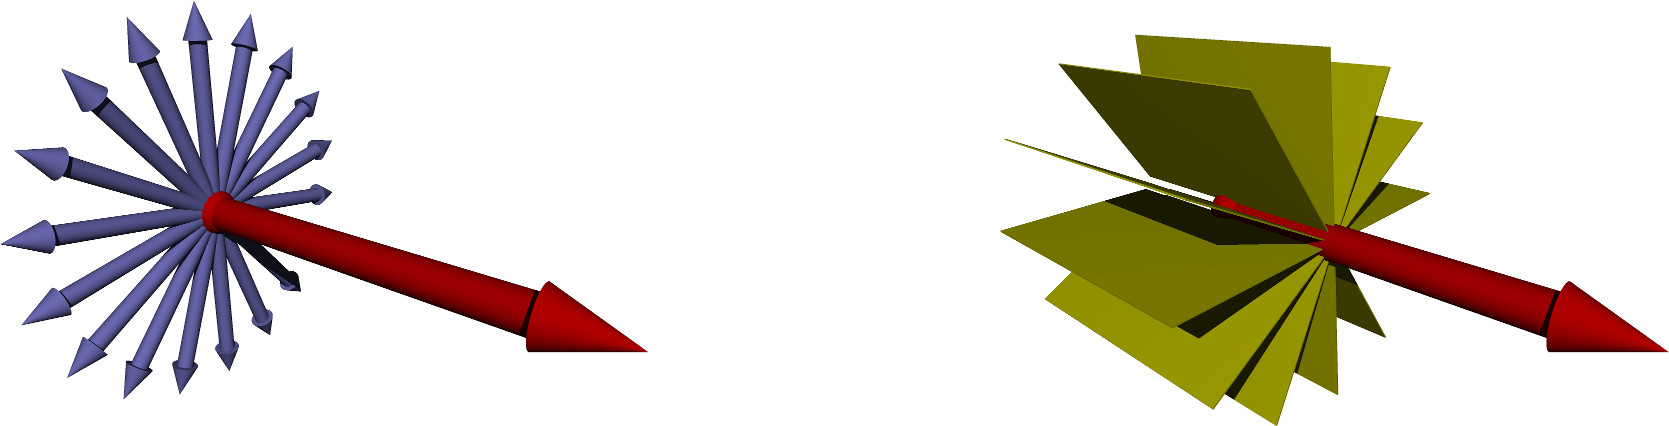
\includegraphics[width=\hsize]{../common/3d/normals.jpg}
\end{center}
\caption{
The normals on the solution surface of quasilinear partial differential
equation of first order are all orthogonal to the vector $\vec{v}$
(red, image on the left).
The tangent planes to the solution surface thus contain the common
direction $\vec{v}$.
\label{geometrie:normals}}
\end{figure}%
Thus the equation \eqref{quasilinear:vektorform} says that the normal
vector $\vec{n}$ is always orthogonal to $\vec{v}$.
We are looking for a surface that has a normal vector orthogonal to
$\vec{v}$.
In each point, there are many planes that have normals orthogonal
to $\vec{v}$, they form a sheaf of planes
(figure~\ref{geometrie:normals}).
Whatever this surface is, the vector $\vec{v}$ must be tangent to
all of them.

So the correct translation of the direction field idea from the 
theory of ordinary differential equations is not to look for a tangent
plane field, but that the equation determines a set of planes
\begin{figure}
\begin{center}
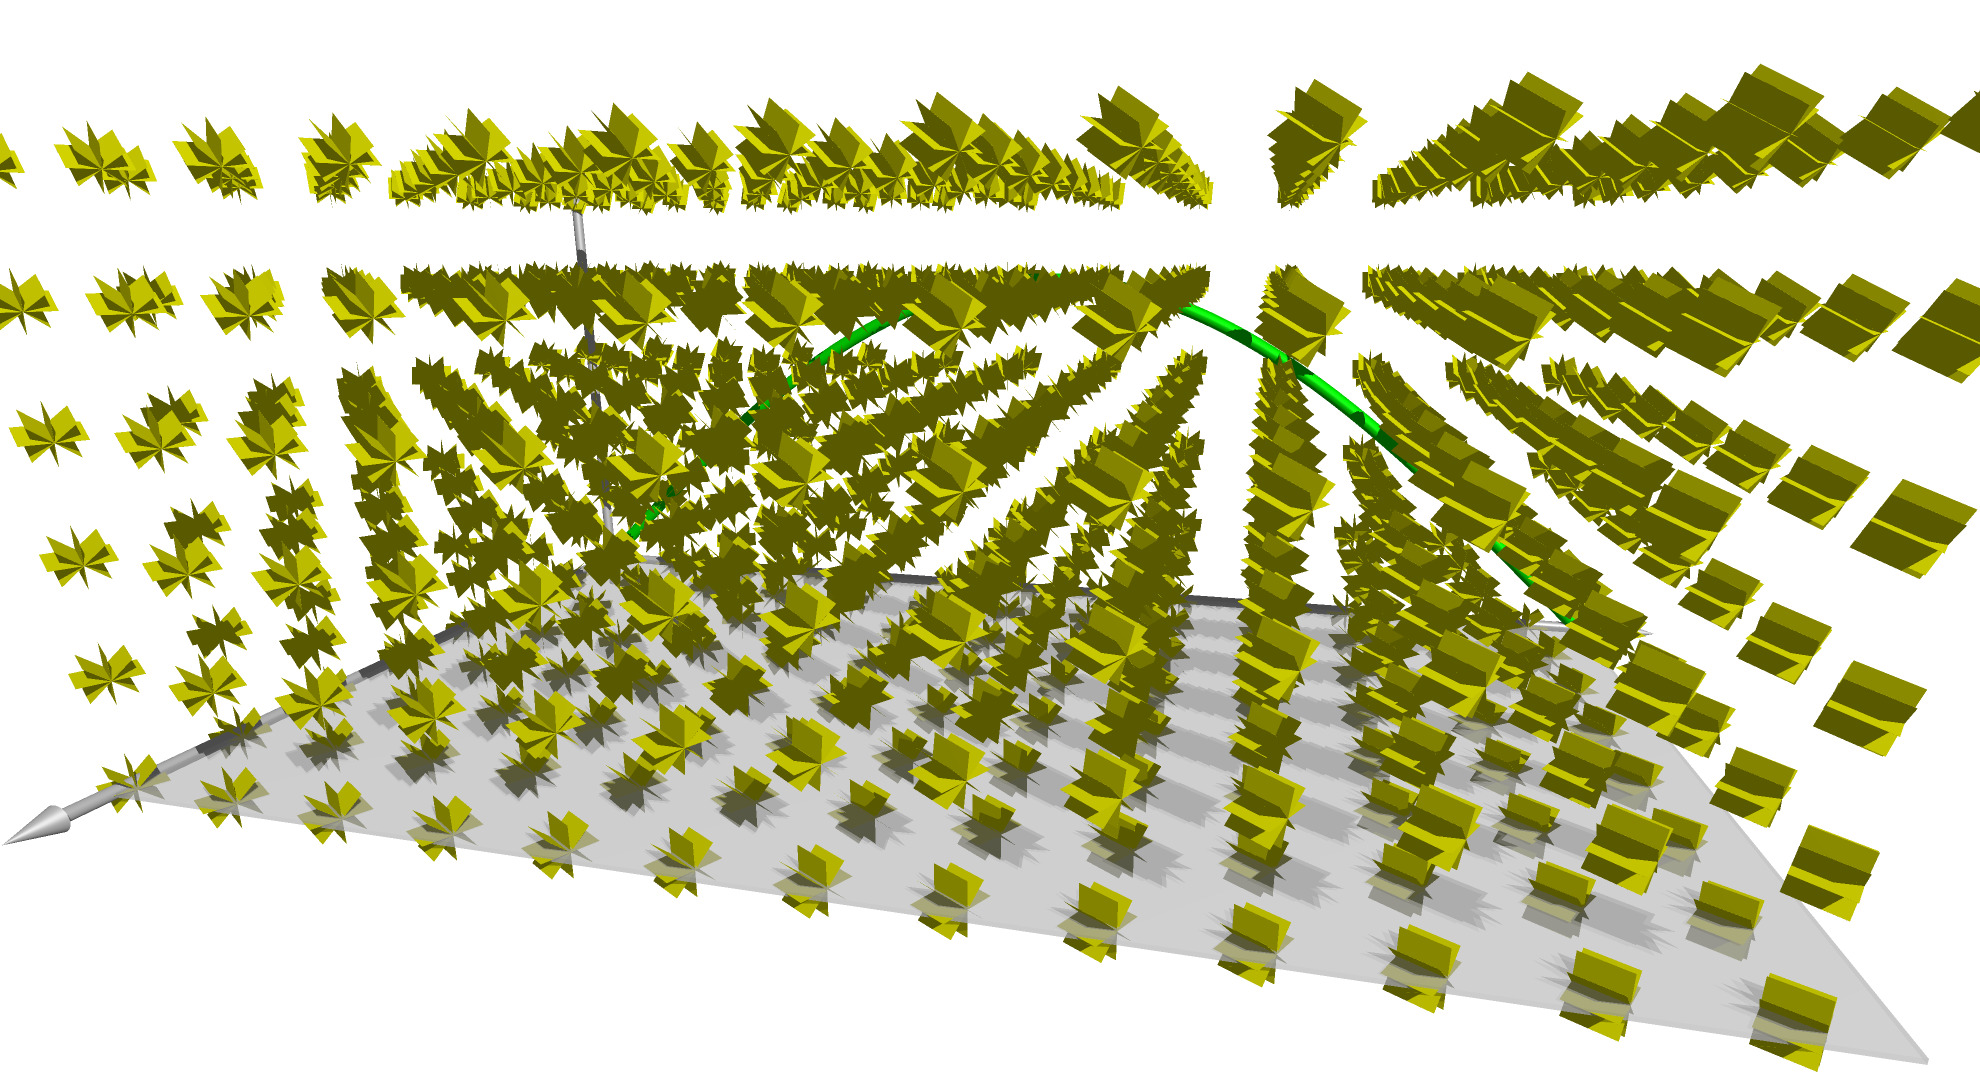
\includegraphics[width=\hsize]{../common/3d/planes.jpg}
\end{center}
\caption{Feld von Ebenenbüscheln, definiert durch eine quasilineare
partielle Differentialgleichung erster Ordnung
\label{geometrie:ebenenbueschelfeld}}
\end{figure}
(figure~\ref{geometrie:ebenenbueschelfeld}), from which the initial
conditions then chooses one.

There are some easy conclusions from this simple observation.
If we have two solution surfaces, then they must always be tangent
to $\vec{v}$.
This means that intersections of solution curves have $\vec{v}$ as their
tangent.
In particular, the vectors
\[
(x,y,u)\mapsto
\vec v=
\begin{pmatrix}
a(x,y,u)\\b(x,y,u)\\c(x,y,u)
\end{pmatrix}
\]
form a vector field that is tangent to the solution surface in any point.

\subsubsection{Characteristics}
To find the solution surface, we now leverage the vector field $\vec{v}$
and try to find the solution it as a set of curves, each of them with
tangent vector $\vec{v}$.
\begin{figure}
\begin{center}
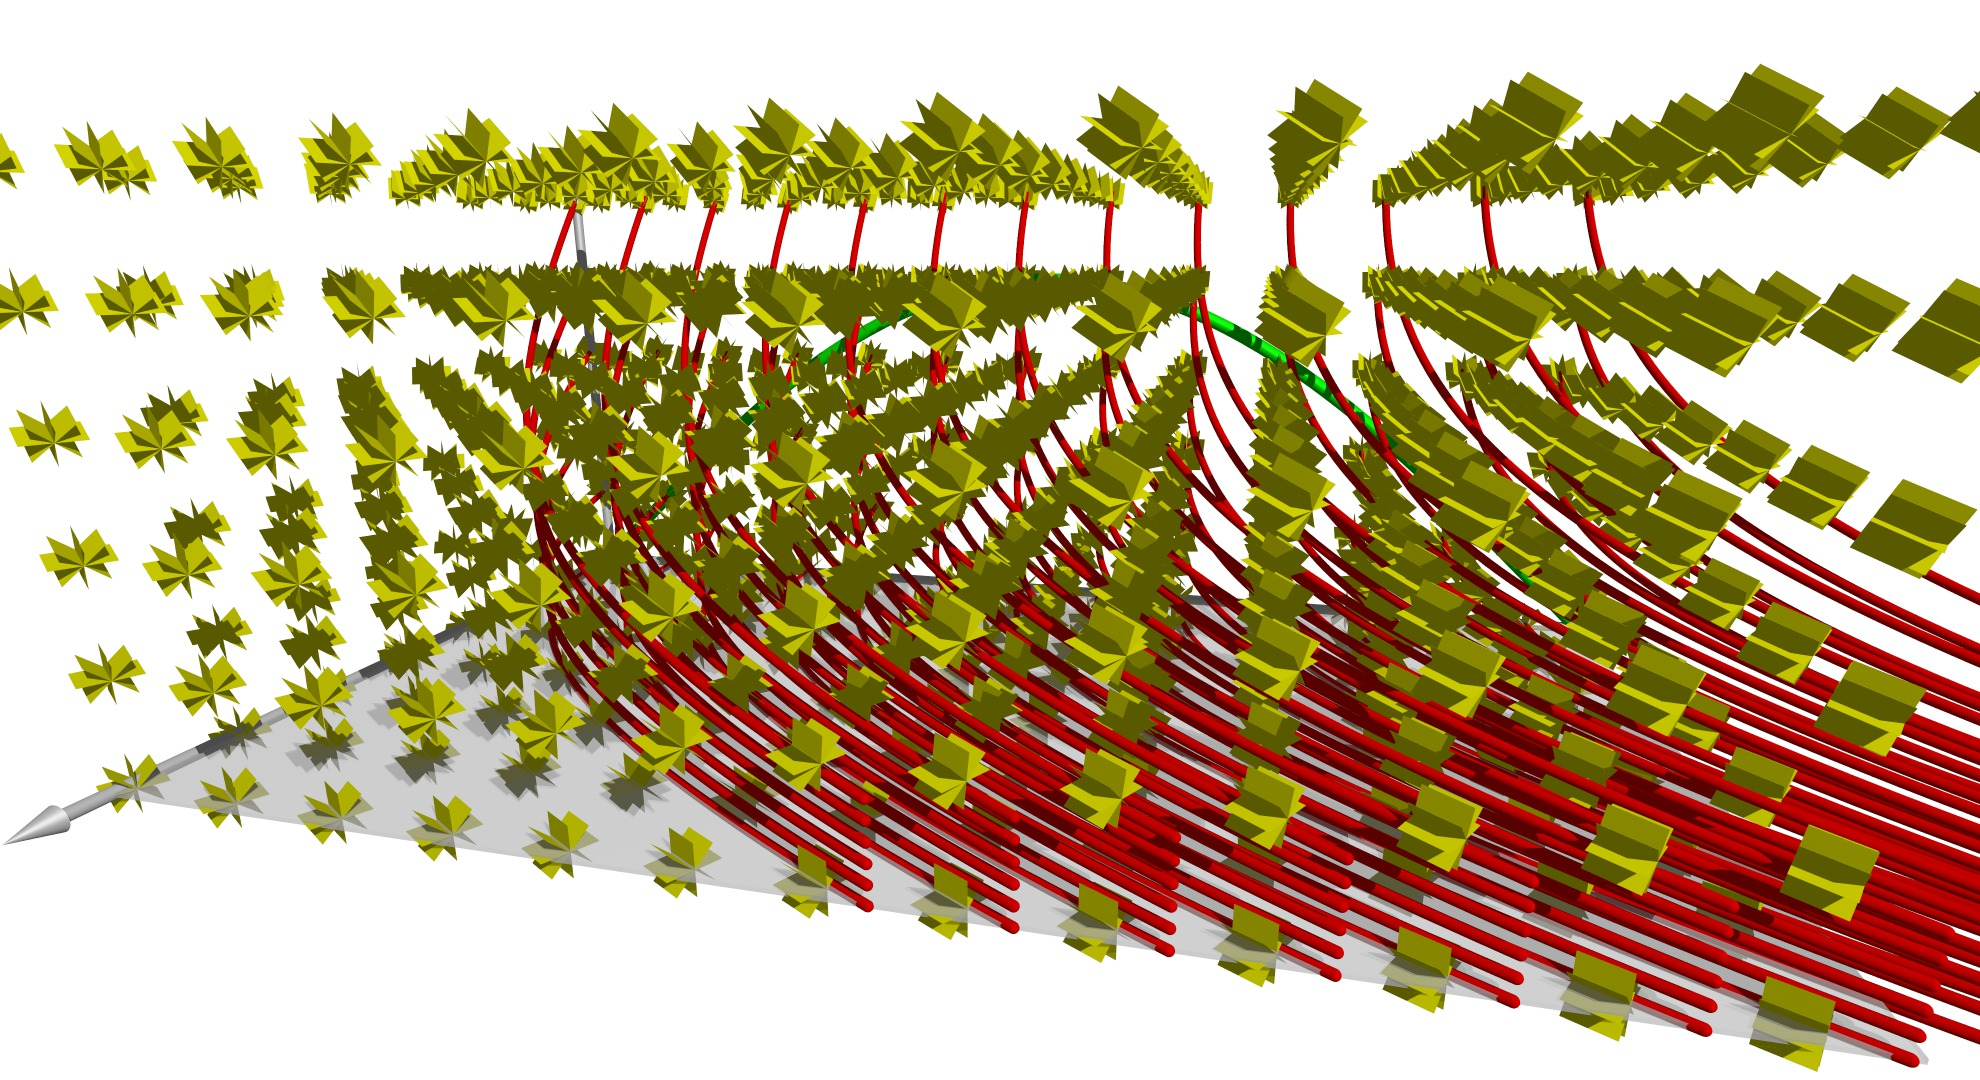
\includegraphics[width=\hsize]{../common/3d/chrpl.jpg}
\end{center}
\begin{center}
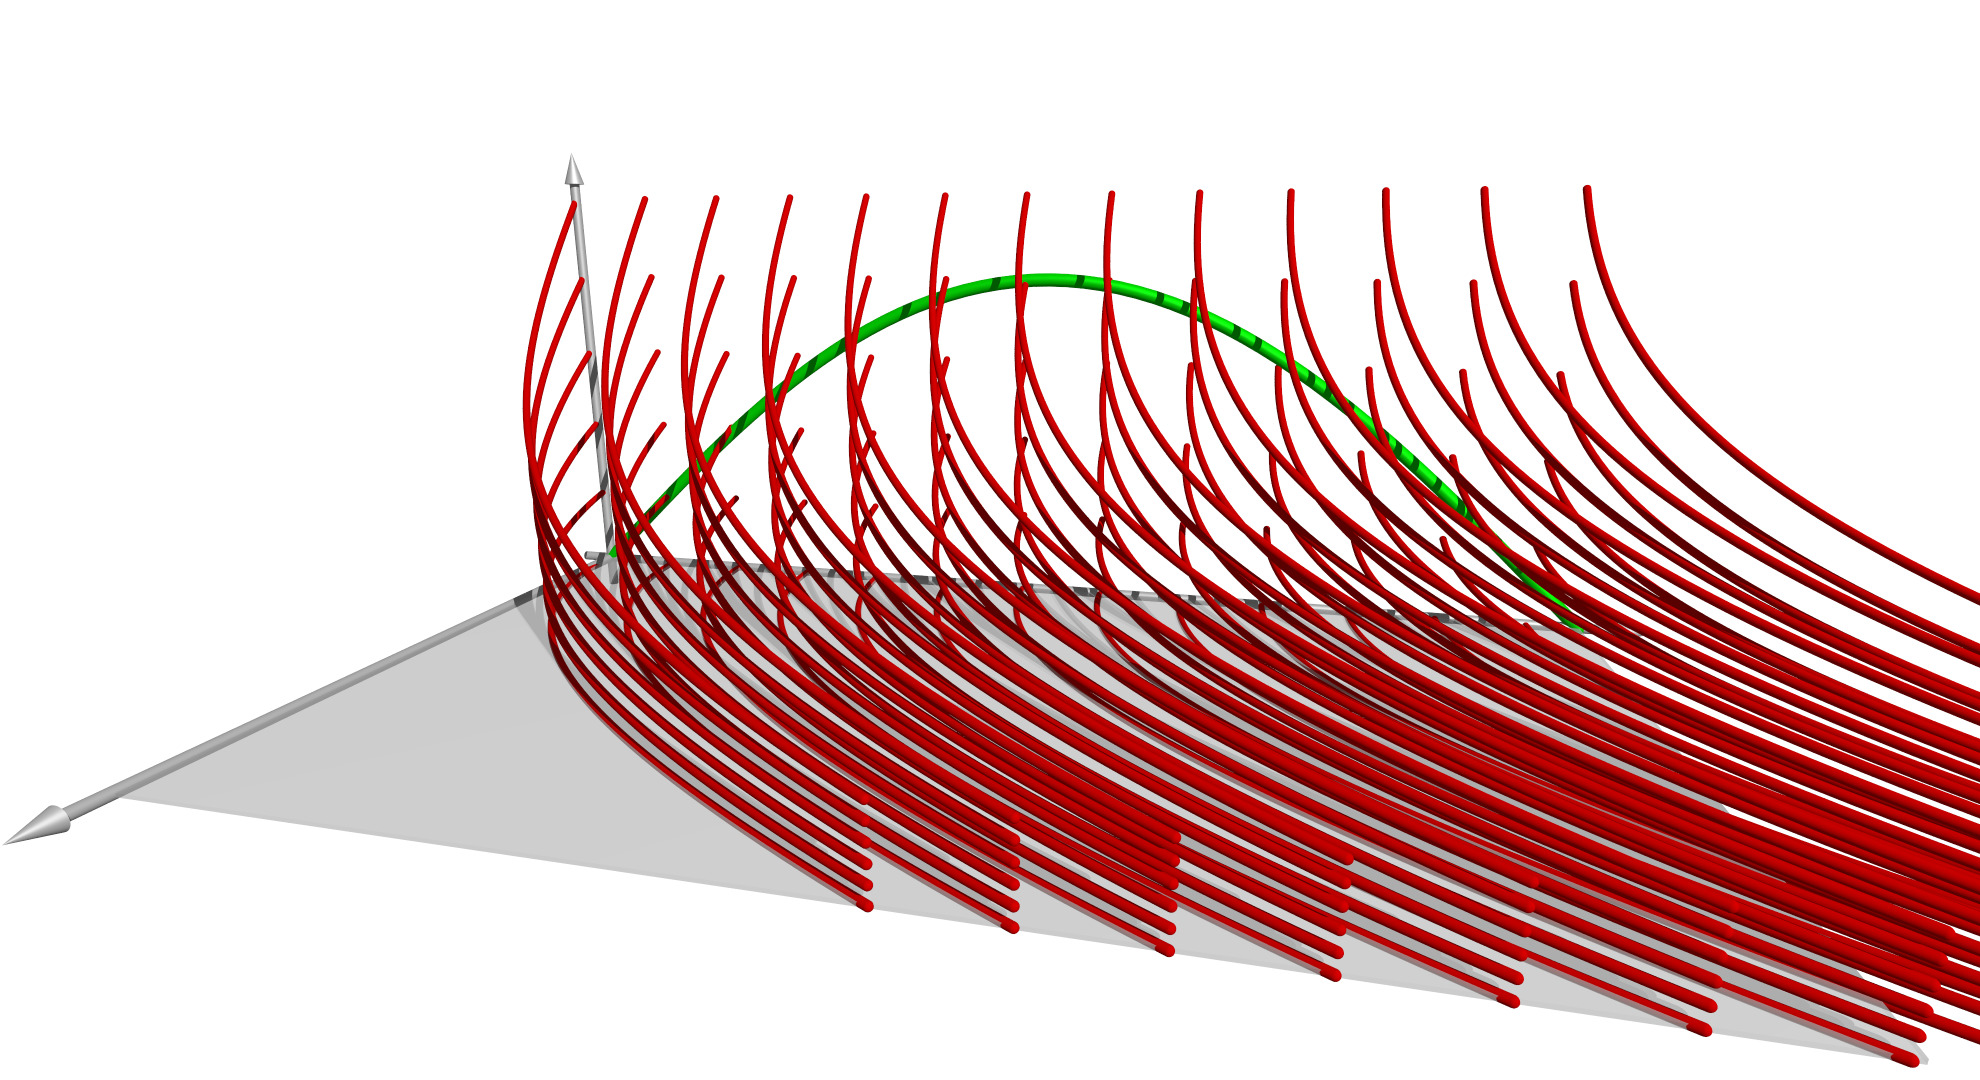
\includegraphics[width=\hsize]{../common/3d/chr.jpg}
\end{center}
\caption{Characteristics of a quasinlinear partiall differential equation
of first order with sheafs of planes (top) and characteristics only (bottom)
\label{geometrie:charekeristiken-mit-buescheln}}
\end{figure}
Given a point on the surface, we can find a solution curve of the vector
field, which will be contained in the surface as well.
To this effect we have to solve the ordinary differential equation
\begin{equation}
\frac{d}{dt}\begin{pmatrix}x(t)\\y(t)\\z(t)\end{pmatrix}
=
\begin{pmatrix}
a(x(t),y(t),u(t))\\b(x(t),y(t),u(t))\\c(x(t),y(t),u(t))
\end{pmatrix}.
\label{quasilinear:charakteristik}
\end{equation}
A solution curve of
\eqref{quasilinear:charakteristik}
is tangential to the solution surface in every point, so it does not
leave the solution surface.

\begin{definition}
\label{def:quasiliniear:charakteristik}
\index{Characteristic!of a  quasilinearen partial
differential equation of first order}
The solution curves of the ordinary differential equations
\eqref{quasilinear:charakteristik} are called {\em characteristics}
of the partial differential equation \eqref{quasilinear:equation}.
\end{definition}

\subsubsection{Solution of the Cauchy problem}
\begin{figure}
\begin{center}
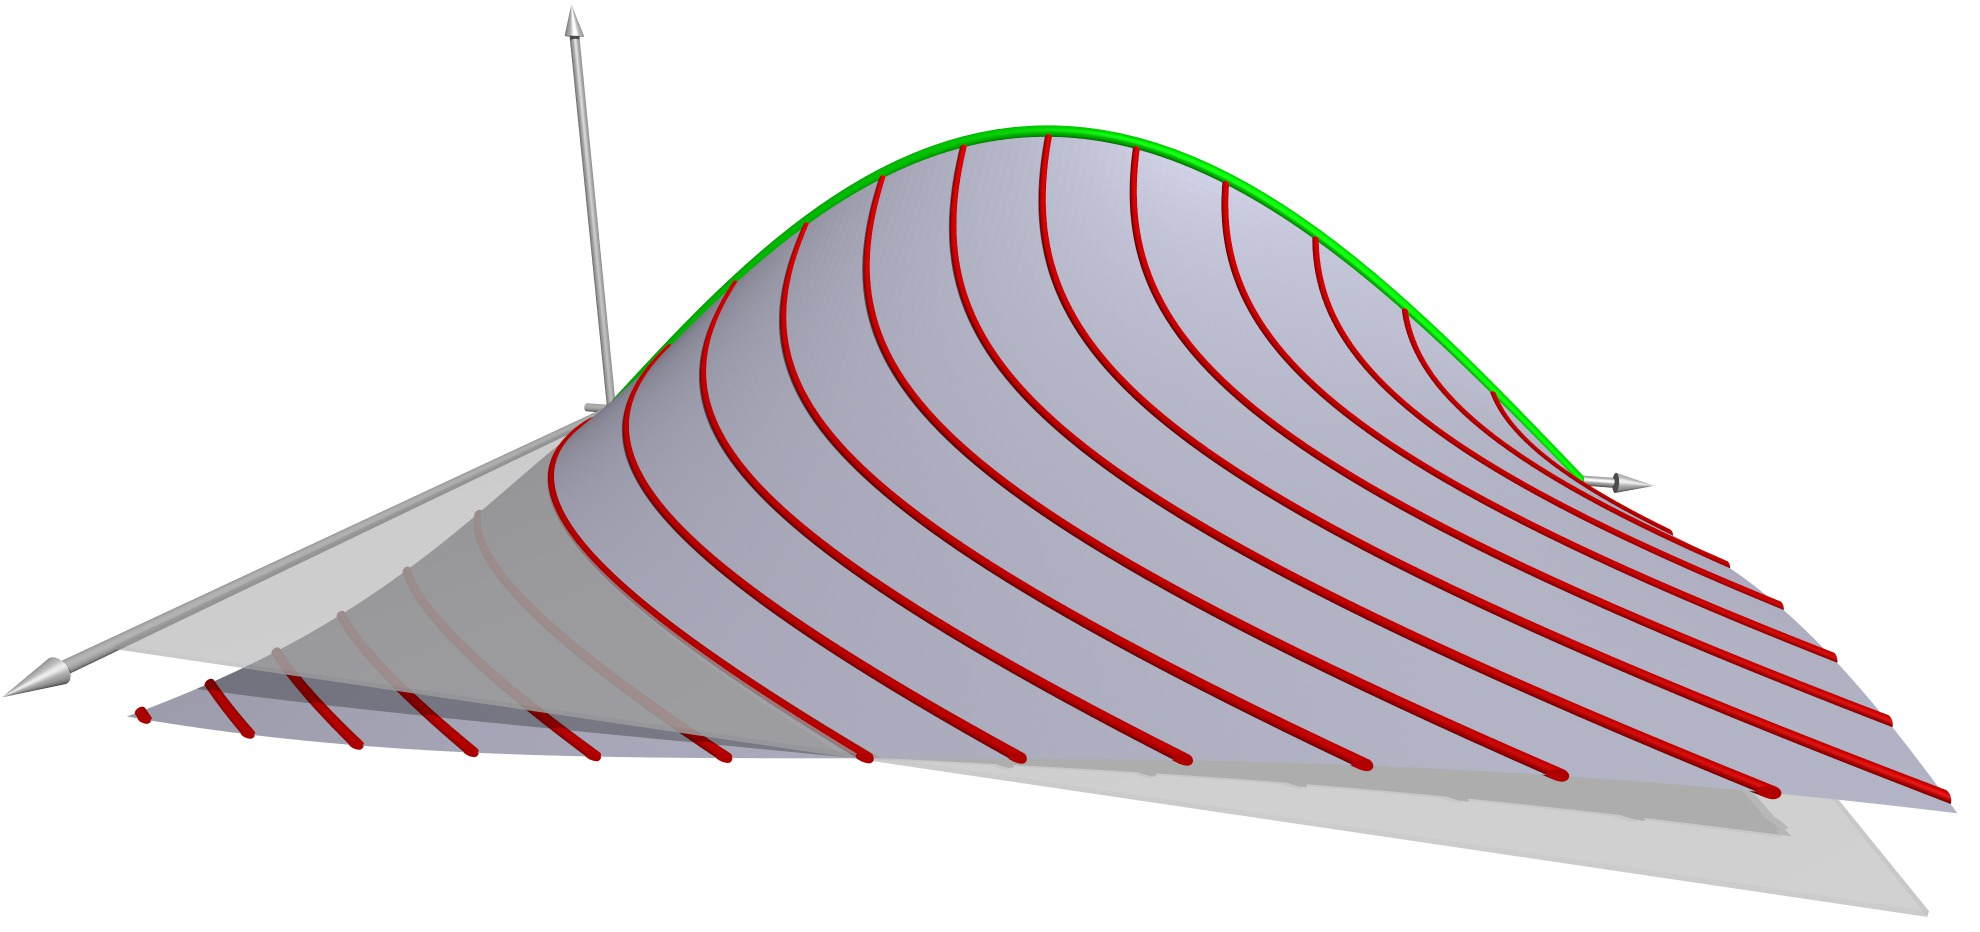
\includegraphics[width=\hsize]{../common/3d/sol.jpg}
\end{center}
\caption{Solution of a quasilinear partial differential equation
of first order: the solution surface is covered by characteristics (red),
they a are parametrized by the parameter of the Cauchy initial curve
(green) and the curve parameter along each characteristic.
\label{geometrie:loesung-mit-charakteristiken}}
\end{figure}
We can now solve the Cauchy problem using characteristics.
The solution surface consists of characteristics which also must
intersect the initial curve
(Abbildung~\ref{geometrie:loesung-mit-charakteristiken}).
To get a solution we thus proceed as follows:
\begin{enumerate}
\item
For each $s$, solve the {\em ordinary} differential equation
\eqref{quasilinear:charakteristik}, which gives a solution curve
$t\mapsto \vec x(s,t)$ with initial condition
$\vec x(s,0)=\vec x_0(s)$.
\item 
Eliminate the parameters $s$ and $t$ from the equations
\eqref{quasilinear:kurvenschar} to find the solution in the form
$z=u(x,y)$.
\end{enumerate}

If the coefficients $a(x,y,u)$, $b(x,y,u)$ and $c(x,y,u)$ are
differential functions, the vector field $\vec{v}$ will be differentiable
as well.
If the initial curve is differentiable, general theorems about dependence
on initial conditions of solutions of ordinary differential equations
state that the solution curve will depend differentiably on $s$.
So the solution found in this way will be differentiable.

In summary we have found a method to reduce a quasilinear partial differential
equation of first order to the solution of a set of ordinary differential
equations.

\subsubsection{Which initial curves work?}
For the solution process just described to work it is imperative that
the initial curve not be a characteristic.
If it was, all the characteristic curves constructed from the initial
curve will coincide with the initial curve.
We don't get a surface but just the initial curve.

The characteristics thus not only give us a method to solve a partial
differential equation but also a method to decide which initial
conditions need to be specified for the solution to actually exist.

Consider a quasilinear partial differential equation on the domain
$\Omega$.
A characteristic emanating from a boundary point with given initial
value at that point will move through the domain but may ultimately
leave it at some other point.
The value of the solution function is already determined at that exit
point by the initial point of the characteristic.
Thus we may not specify this boundary value independently, or the
partial differential equation may not have a solution at all.

Thus boundary values need to be specified on a subset
$M\subset\partial \Omega$ of the domain such that all the
characteristics covering $\Omega$ meet $M$ in exactly one point.

\subsection{Examples}
In this section we compute a few examples for the solution procedure
discussed above.

\subsubsection{Constant coefficients
\label{konstantekoeff}}
We want to solve the Cauchy problem for the partial differential equation
\[
\frac{\partial u}{\partial x}+2\frac{\partial u}{\partial y}=3
\]
with boundary values $u(0,y)=\sin y$ in the domain $x>0$.

The initial curve parametrized by $s$ has the form
\[
\vec x_0(s)
=
\begin{pmatrix}
0\\s\\\sin s
\end{pmatrix}.
\]
Now we have to find a set of ``red'' curves emanating from this 
initial curve.

The ordinary differential equation for the characteristics is
\[
\frac{d}{dt}\begin{pmatrix}x(t)\\y(t)\\z(t)\end{pmatrix}
=
\begin{pmatrix}1\\2\\3\end{pmatrix}.
\]
It has the solution curves
\[
t\mapsto\begin{pmatrix}x_0\\y_0\\z_0\end{pmatrix}+t\begin{pmatrix}1\\2\\3\end{pmatrix}.
\]
The initial point
$(0,s,\sin s)$
thus progresses in time $t$ to
\[
\begin{pmatrix}
x(s,t)\\
y(s,t)\\
z(s,t)
\end{pmatrix}
=
\begin{pmatrix}0\\s\\\sin s\end{pmatrix}+t\begin{pmatrix}1\\2\\3\end{pmatrix}
=
\begin{pmatrix}
t\\
s+2t\\
\sin s+3t
\end{pmatrix}.
\]
This set of curves describes the solution surface with parameters $s$ and $t$,
we prefer a solution in the more familiar form $u(x,y)$.
To this effect, we have to eliminate $s$ and $t$ from the equations
\begin{align*}
x&=t\\
y&=s+2t\\
z&=\sin s+3t.
\end{align*}
The first equation means that we can replace $t$ by $x$.
The second equation then reduces to $s=x-2x$.
Replacing $s$ in the third equation then gives $z=\sin(y-2x)+3t$.
So the solution is
\[
u(x,y)=\sin(y-2x)+3x.
\]
By substituting this expression into the partial differential equation
and into the boundary condition, one can verify that it is in fact a 
solution:
\begin{align*}
\frac{\partial u}{\partial x}
&=-2\cos(y-2x)+3
\\
\frac{\partial u}{\partial y}
&=\cos (y-2x)
\\
\Rightarrow\qquad
\frac{\partial u}{\partial x}
+2
\frac{\partial u}{\partial y}
&=
-2\cos(y-2x)+3
+2\cos(y-2x)=3
\\
u(0,y_0)&=\sin y_0.
\end{align*}

\subsubsection{Circular Characteristics}
The differential equation for the characteristics can lead to very 
complicated curves in the domain with serious repercussions on the
existence of solutions are boundary conditions that actually permit
a solution.
To illustrate this, the following example exhibits characteristics, that
have circles as projection into the $x$-$y$-plane.

We solve the partial differential equation
\[
y\frac{\partial u}{\partial x}-x\frac{\partial u}{\partial y}=0.
\qquad\Omega=\{(x,y)\,|x>0\}
\]
It obviously is linear, thus the method of characteristics applies.
We have to find solution curves of the vector field
\[
\begin{pmatrix}
y\\-x\\0
\end{pmatrix}.
\]
Since the $z$-component of $\vec{v}$ vanishes, the $z$-component of the
solution curves will also be constant and we can ignore it for the
following computation and concentrate on $x$ and $y$.

Solution curves for the vector field
\[
\begin{pmatrix}
y\\-x
\end{pmatrix}
\]
in the plane are functions $x(t)$ and $y(t)$ which satisfy the equations
\begin{align*}
\dot x(t)&=y(t)\\
\dot y(t)&=-x(t).
\end{align*}
Taking the derivative of the first equation ans substituting it into
the second equation gives the differential equation of second order
\[
\ddot x(t)=-x(t)
\]
with well known solutions $a\cos t$ and $b \sin t$.
For $t=0$ the curve must start on the $x$-Axis, which rules out the
cosine solution.
As a consequence, the solution curve in vector notation is
\[
\begin{pmatrix}
x(t)\\y(t)
\end{pmatrix}
=y_0\begin{pmatrix}
\sin t\\
\cos t
\end{pmatrix}.
\]
These curves are circles around the origin with radius $y_0$.
So we are exactly in the situation where a characteristic starting on
the negative $y$-axis leaves the domain through a point on the positive
$y$-axis.
This means that it sufficies to specify initial conditions for $y_0<0$.

We can now find a formula for the solution with bondary condition $g(y)$
as follows.
For each point $(x,y)$ we have to find $y_0$ and $t$.
Obviously, $|y_0|$ is the radius of the point so we can write
\[
y_0 = -\sqrt{x^2+y^2}.
\]
Since $u$ does not depend on $t$, this is sufficient to determine
the value of $u(x,y)$:
\[
u(x,y)=g(-\sqrt{x^2+y^2}).
\]

Here are some conclusions we can draw from this example:
\begin{enumerate}
\item
Dass Festlegung einer Anfangsbedingung für $y_0>0$ nicht nötig ist,
kann man der Differentialgleichung in unmittelbarer Nähe der $y$-Achse nicht
ansehen, erst der Verlauf der Charakterisitiken im Grossen ermöglicht
diese Erkenntnis. Dieses Phänomen wird durch den ``zusätzlichen Platz''
ermöglicht, den der zweidimensionale Definitionsbereich der partielle Differentialgleichung gegenüber dem
eindimensionalen Definitionsbereich der gewöhnlichen DGL bietet.
\item
The point $(0,0)$ has special properties.
If the solution is supposed to be continuous, we need
$g(0)=\lim_{y\to 0-} g(y)$, so $g$ must be left continuous in $0$.
For the solution to be differentiable, we need $g'(x)=0$ in addition
to that.
\end{enumerate}

\subsubsection{Ein nicht lösbares Anfangswertproblem\label{unloesbar}}
There are multiple scenarios where the method of characteristics can 
show that a partial differential equation cannot be solved.
This examples serves to illustrate one such scenario.

The partial differential equation
\[
x\frac{\partial u}{\partial x}
+
y\frac{\partial u}{\partial y}
=0
\]
is to be solved with boundary conditions
$u(0,y)=\sin y$
in $\Omega=\{(x,y)\,|\, x>0\}$.
We again first determine the characteristics (without the $z$-component,
which, as before, is constant)
\[
\frac{d}{dt}
\begin{pmatrix}
x(t)\\y(t)
\end{pmatrix}
=
\begin{pmatrix}
x(t)\\y(t)
\end{pmatrix}
\quad
\Rightarrow
\quad
\left\{
\begin{aligned}
\dot x(t)&=x(t)\\
\dot y(t)&=y(t)
\end{aligned}
\right.
\]
Thus the solution curves are straight lines through the origin:
\[
\begin{pmatrix}
x(t)\\y(t)
\end{pmatrix}
=\begin{pmatrix}x_0\\y_0\end{pmatrix}e^t
\]
To construct a solution, we have to find the point from which the 
characteristic curve through the point $(x,y)$ emanates.
But since all characteristics go through the origin, this will always
be the origin.
All function values are determined by the boundary value in $(0,0)$.

The problem of course stems from the fact that $y$-axis is a characteristic.
We have seen previously that characteristics can be characterized as the
curves not suitable as initial curves.

\subsection{General partial differential equation of first order}
Let's examine the following more general partial differential equation of first
order for an unknown function $u(x,y)$
\begin{equation}
F\biggl(
x,y,u(x,y),\frac{\partial u}{\partial x},\frac{\partial u}{\partial y}
\biggr)=0.
\label{skript:generalpde}
\end{equation}
This equation describes an explicit relation between location in
$x$-$y$-$u$-space and slopes 
$\partial_xu$ and $\partial_yu$.

A boundary value problem for initial values along the $y$-axis
$x=0$ specifies boundary values with a function $g(y)$ as
\[
u(0,y)=g(y).
\]
This also specifies the partial derivatives with respect to $y$.
The partial differential equation \eqref{skript:generalpde} then
limits the possible values for the partial derivatives
$\partial_xu(0,y)$.
In some cases this partial derivative will not be determined uniquely.
If it does, then as before, we can conclude that the Cauchy problem 
has unique solutions.

However, it is no longer so simple to determine which initial values
need to be specified, as the derivation of the method characteristics
critically depends on the equation being quasilinear.
The concept of characteristics is no longer applicable.


